\ProvidesFile{ch-background-signals.tex}[Background Signals]
\chapter{Background Signals}
\graphicspath{{/Users/liamrobinson/Documents/PyLightCurves/docs/build/html/_images}}

Whenever an optical telescope is observing a space object, the object's signal is necessarily superimposed on whatever signals exist in the background. In this context, background does not only refer to sources physically further than the object, but all sources that impact the image apart from the object signal. As we will see, some of these sources even originate within the telescope. To faithfully simulate a telescope observing an object, many position-based SDA tasks are able to ignore background effects while acquiring or tracking objects. For photometry-based SDA, the background is critical. Background signals can be broken up into atmospheric effects, exoatmospheric effects, and sensor effects. 

\section{Atmospheric Effects}

\subsection{Airglow}

Certain chemical reactions from 80-110 km altitude in the upper atmosphere release visible light
\cite{krag2003}. This effect is known as
airglow. Since these reactions are assumed to be isotropic ---  equally intense when integrated along any
vertical line extending upwards from the surface. We model the airglow signal $\textrm{AINT}$ in a
similar fashion to integrated starlight. Given the airglow spectra $\textrm{GLINT}(\lambda) \:
\left[ \frac{W}{m^2\cdot m \cdot rad^2} \right]$, we compute Eq \ref{eq:aint}.

\begin{equation} \label{eq:aint}
 \textrm{AINT} = \frac{\pi D^2}{4}
  \int_{10^{-8}}^{10^{-6}}{ \textrm{GLINT}(\lambda) \cdot \textrm{QE}(\lambda) \cdot \textrm{ATM}(\lambda)
  \cdot \left( \frac{\lambda}{h c} \right) \: d\lambda}  
\end{equation}

The quantity $\textrm{AINT}$ has units $\left[ \frac{1}{s\cdot rad^2} \right]$, meaning that the
airglow signal in ADU is simply given by Eq \ref{eq:airglow_adu}

\begin{equation} \label{eq:airglow_adu}
van_rhijn
\end{equation}

In Eq \ref{eq:airglow_adu}, $\frac{1}{\cos(\theta_z)}$ is known as the Van Rhijn factor, which
accounts for the accumulation of airmass near the horizon \ref{frueh2019}.

\begin{figure}[ht]
  \centering
  \includegraphics[width=\figmed]{sphx_glr_background_signals_005.png}
  \caption{Airglow signal on the local observer hemisphere. The observer is in New Mexico, USA at
  \pogslla}
  \label{fig:airglowhemi}
\end{figure}

\subsection{Light Pollution}

The final source of background noise light pollution. On a cloudless night with negligible light
pollution, the zenith surface brightness is approximately $22 \: \left[ \frac{mag}{arcsec^2}
\right]$ \cite{krag2003}. As light pollution increases, this zenith brightness may dip down to
$14-15 \: \left[ \frac{mag}{arcsec^2} \right]$. To get accurate localized zenith brightness values,
we use the 2015 World Atlas of Sky Brightness \cite{falchi2016_data}. The data is reported in $\left[
	\frac{mcd}{m^2} \right]$

\begin{figure}[ht]
  \centering
  \includegraphics[width=\figmed]{sphx_glr_background_signals_006.png}
  \caption{Light pollution signal on the local observer hemisphere. The observer is in New Mexico, USA at
  \pogslla}
  \label{fig:pollutionhemi}
\end{figure}

\section{Exoatmospheric Effects}

\subsection{Integrated Starlight}

Stars are almost always present in optical images of space objects. The brightest stars streaking across the field of view in REFFIGBELOW have high SNRs and stand out clearly against the dark background. This raises a question: if we're observing a full $1^\circ \times 1^\circ$ area of the sky, where are the rest of the stars given that the Milky Way alone contains approximately $1\cdot10^{11}$ stars? The answer is relatively obvious: many more stars are present in the image than we can pick out individually, most of them fall into the background. We call this residual faint starlight "integrated" starlight as we are effectively integrating the signals from thousands or millions of stars across the image plane. 

\begin{figure}[ht]
  \centering
  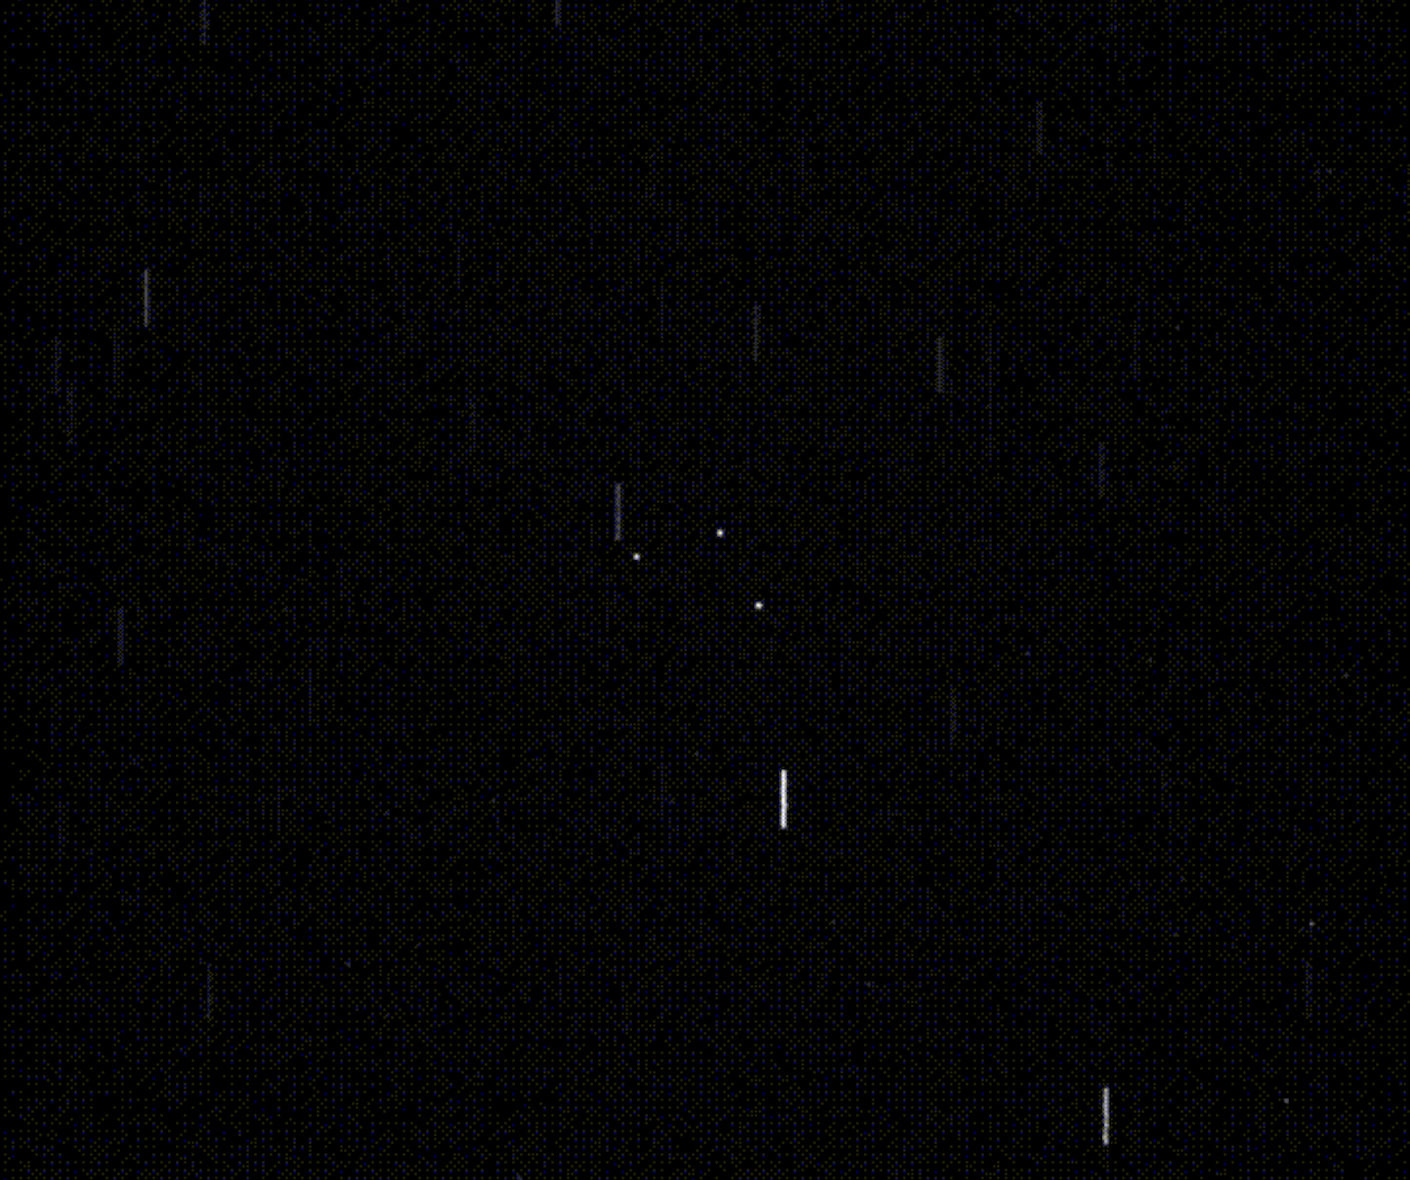
\includegraphics[width=\figmed]{static_images/static_pogs_raw_image.png}
  \caption{Raw image of three GEO objects with stars streaking through the background. Taken by the Purdue Optical Ground station at \pogslla by Nathan Houtz}
  \label{fig:pollutionhemi}
\end{figure}

Most stars are too faint to appear as points of light on the image plane. Instead, they merge
into the background. The signal due to these faint stars is known as integrated starlight.
Krag \cite{krag2003} modeled this signal by building a $1^\circ \times 1^\circ$ grid of surface
brightness values for the full right ascension (RA) and declination (Dec) sphere. Krag used the
Guide Star catalog, which contains 15 million stars down to magnitude 16. Exponential extrapolation
was used to predict star counts in each bin for higher magnitudes \cite{krag2003}. Twenty years later, we have
access to larger star catalogs that are nearly complete to much dimmer magnitudes. The integrated
starlight catalog used in this work was built from the GAIA catalog with approximately 1.5 billion
stars down to magnitude 21-22 \cite{gaia_dr3}. The same $1^\circ \times 1^\circ$ grid was computed
using the \texttt{astroquery.gaia} Python package \cite{astroquery_gaia}. Figure
\ref{fig:gaiapatched} shows the computed patched catalog, in units of $S_{10}$. 

\begin{figure}[ht]
  \centering
  \includegraphics[width=\figbig]{sphx_glr_gaia_patched_catalog_001_2_00x.png}
  \caption{Integrated starlight patched catalog}
  \label{fig:gaiapatched}
\end{figure}

Now that we have a data source for the exoatmospheric mean brightness of the night sky due to integrated
starlight, we can compute the corresponding signal mean for a telescope equipped with a CCD sensor.
Again, we adopt Krag's formulation \cite{krag2003}.

\begin{equation} \label{eq:bint}
 \textrm{BINT} = \frac{\pi D^2}{4}
  \int_{10^{-8}}^{10^{-6}}{ \textrm{STRINT}(\lambda) \cdot \textrm{QE}(\lambda) \cdot \textrm{ATM}(\lambda)
  \cdot \left( \frac{\lambda}{h c} \right) \: d\lambda}  
\end{equation}

In Eq \ref{eq:bint}, $D$ is the telescope aperture diameter in meters, $h$ is Plank's constant in
$\left[ \frac{m^2 kg}{s} \right]$, and $c$
is the speed of light in vacuum in $\left[ \frac{m}{s} \right]$. The resulting quantity
$\textrm{BINT}$ has units of $\left[ \frac{1}{s} \right]$, representing the mean total photons passing
through the telescope aperture due to integrated starlight. 

\begin{equation} \label{eq:starlightmean}
  \bar{S}_{star} = 10^{-4} \cdot BINT \cdot \left( \frac{s}{3600} \right)^2 \cdot \Delta t \cdot
  b_{cat}
\end{equation}

In Eq \ref{eq:starlightmean}, $b_{cat}$ is the patched catalog brightness in $\left[ S_{10}
\right]$, $s$ is the telescope pixel scale in $\left[ \frac{arcsecond}{pix} \right]$, and $\Delta t$ is the integration time in seconds. Note the addition of the $10^{-4}$ factor to reconcile catalog surface brightness in terms of 10th magnitude stars, and the 0th magnitude source in $\textrm{BINT}$. This yields $\bar{S}_{star}$ with units $\left[ \frac{e^-}{pix^2} \right]$; photoelectron counts per pixel area. Figure \ref{fig:starlighthemi} shows the background signal mean due to integrated starlight.

\begin{figure}[ht]
  \centering
  \includegraphics[width=\figmed]{sphx_glr_background_signals_002.png}
  \caption{Integrated starlight signal on the local observer hemisphere. The observer is in New Mexico, USA at
  \pogslla}
  \label{fig:starlighthemi}
\end{figure}

\subsection{Scattered Moonlight}

\begin{figure}[ht]
  \centering
  \includegraphics[width=\figmed]{sphx_glr_background_signals_001.png}
  \caption{Scattered moonlight signal on the local observer hemisphere. The observer is in New Mexico, USA at
  \pogslla}
  \label{fig:moonlighthemi}
\end{figure}

\subsection{Zodiacal Light}

\section{Sensor Effects}

\subsection{Dark Noise}
\subsection{Readout Noise}
